\documentclass{beamer}

\mode<presentation>
{
   \usetheme{EEng}
%   \usetheme{Warsaw}
  \setbeamercovered{transparent}
  \setbeamercolor{background canvas}{bg=black!0}
}

\usepackage{enumerate}
\usepackage{array}
\usepackage{graphics}
\usepackage{ucs}
\usepackage[utf8x]{inputenc}
\usepackage[english]{babel}
\usepackage{amsmath, amsthm, amssymb}
\usepackage{amsmath}
\usepackage{amsfonts}
\usepackage{xcolor}
\usepackage{pgf}
\usepackage{hyperref}
\usepackage{url}
\usepackage{multicol}   % add-on
\usepackage{boxedminipage} 
\usepackage{indentfirst}   % add-on
\usepackage{float}
\usepackage{listings}
\usepackage{verbatim}
\usepackage{boxedminipage}
\usepackage{haskell}

% % % inicio do listings e ref
\definecolor{darkblue}{rgb}{0,0,0.6}
\definecolor{gray_ulisses}{gray}{0.55}
\definecolor{castanho_ulisses}{rgb}{0.71,0.33,0.14}
\definecolor{preto_ulisses}{rgb}{0.41,0.20,0.04}
\definecolor{green_ulises}{rgb}{0.2,0.75,0}

\hypersetup{
	a4paper,
	pdftex,
	bookmarks,
	colorlinks,
    citecolor=darkblue,
    linkcolor=darkblue,
    urlcolor=darkblue,
    filecolor=darkblue
}

\lstdefinelanguage{Terminall} {
       basicstyle=\scriptsize\ttfamily,
       breaklines=true,
       breakautoindent=false,
       showstringspaces=false
}
\lstnewenvironment{code_files}{\lstset{language=Terminall}}{}

\lstdefinelanguage{Terminal} {
       basicstyle=\tiny\ttfamily,
       breaklines=true,
       breakautoindent=false,
       showstringspaces=false
}
\lstnewenvironment{code}{\lstset{language=Terminal}}{}

\definecolor{gray_ulisses}{gray}{0.55}
\definecolor{castanho_ulisses}{rgb}{0.71,0.33,0.14}
\definecolor{preto_ulisses}{rgb}{0.41,0.20,0.04}
\definecolor{green_ulises}{rgb}{0.2,0.75,0}

\lstdefinelanguage{HaskellUlisses}
{
        basicstyle=\ttfamily\tiny,
        %backgroundcolor=\color{yellow},
        %frameshape={RYRYNYYYY}{yny}{yny}{RYRYNYYYY}, %contornos... muito nice...
        sensitive=true,
        morecomment=[l][\color{gray_ulisses}\ttfamily\tiny]{--},
        morecomment=[s][\color{gray_ulisses}\ttfamily\tiny]{\{-}{-\}},
        morestring=[b]",
        stringstyle=\color{red},
        showstringspaces=false,
%       numbers=left,
%       firstnumber=\thelstnumber,
        numberstyle=\tiny,
        numberblanklines=true,
        showspaces=false,
        breaklines=true,
        showtabs=false,
%       xleftmargin=15pt,
%       xrightmargin=-20pt,
        emph=
        {[1]
                FilePath,IOError,abs,acos,acosh,all,and,any,appendFile,approxRational,asTypeOf,asin,
                asinh,atan,atan2,atanh,basicIORun,break,catch,ceiling,chr,compare,concat,concatMap,
                const,cos,cosh,curry,cycle,decodeFloat,denominator,digitToInt,div,divMod,drop,
                dropWhile,either,elem,encodeFloat,enumFrom,enumFromThen,enumFromThenTo,enumFromTo,
                error,even,exp,exponent,fail,filter,flip,floatDigits,floatRadix,floatRange,floor,
                fmap,foldl,foldl1,foldr,foldr1,fromDouble,fromEnum,fromInt,fromInteger,fromIntegral,
                fromRational,fst,gcd,getChar,getContents,getLine,head,id,inRange,index,init,intToDigit,
                interact,ioError,isAlpha,isAlphaNum,isAscii,isControl,isDenormalized,isDigit,isHexDigit,
                isIEEE,isInfinite,isLower,isNaN,isNegativeZero,isOctDigit,isPrint,isSpace,isUpper,iterate,
                last,lcm,length,lex,lexDigits,lexLitChar,lines,log,logBase,lookup,map,mapM,mapM_,max,
                maxBound,maximum,maybe,min,minBound,minimum,mod,negate,not,notElem,null,numerator,odd,
                or,ord,otherwise,pi,pred,primExitWith,print,product,properFraction,putChar,putStr,putStrLn,quot,
                quotRem,range,rangeSize,read,readDec,readFile,readFloat,readHex,readIO,readInt,readList,readLitChar,
                readLn,readOct,readParen,readSigned,reads,readsPrec,realToFrac,recip,rem,repeat,replicate,return,
                reverse,round,scaleFloat,scanl,scanl1,scanr,scanr1,seq,sequence,sequence_,show,showChar,showInt,
                showList,showLitChar,showParen,showSigned,showString,shows,showsPrec,significand,signum,sin,
                sinh,snd,span,splitAt,sqrt,subtract,succ,sum,tail,take,takeWhile,tan,tanh,threadToIOResult,toEnum,
                toInt,toInteger,toLower,toRational,toUpper,truncate,uncurry,undefined,unlines,until,unwords,unzip,
                unzip3,userError,words,writeFile,zip,zip3,zipWith,zipWith3,listArray,doParse
        },
        emphstyle={[1]\color{blue}},
        emph=
        {[2]
                Bool,Char,Double,Either,Float,IO,Integer,Int,Maybe,Ordering,Rational,Ratio,ReadS,ShowS,String,
                Word8,InPacket
        },
        emphstyle={[2]\color{castanho_ulisses}},
        emph=
        {[3]
                case,class,data,deriving,do,else,if,import,in,infixl,infixr,instance,let,
                module,of,primitive,then,type,where
        },
        emphstyle={[3]\color{preto_ulisses}\textbf},
        emph=
        {[4]
                quot,rem,div,mod,elem,notElem,seq
        },
        emphstyle={[4]\color{castanho_ulisses}\textbf},
        emph=
        {[5]
                EQ,False,GT,Just,LT,Left,Nothing,Right,True,Show,Eq,Ord,Num
        },
        emphstyle={[5]\color{preto_ulisses}\textbf}
}
\lstnewenvironment{haskellcode}{\lstset{language=HaskellUlisses}}{}
% % % fim do listings e ref

% % % inicio da definicao de comandos

% % % fim da definicao de comandos

\title{SOPAS - Submissão Online Para Análise de Software (fase 4)}
\author{José Pedro Silva \and
Pedro Faria \and
Ulisses Costa
}

\date{\today}
\institute{Engenharia de Linguagens\\
Projecto integrado
}

\AtBeginSubsection[] {
  \begin{frame}<beamer>
    \frametitle{Index}
    \scriptsize{\tableofcontents[currentsection,currentsubsection]}
  \end{frame}
}

\AtBeginSection[] {
  \begin{frame}<beamer>
    \frametitle{Index}
    \scriptsize{\tableofcontents[currentsection]}
  \end{frame}
}
\begin{document}
\begin{frame}
   \titlepage
\end{frame}

\section{Objectivos}
\begin{frame} \frametitle{Até agora:}
Concretizado até ao ínicio da quarta fase:
\begin{itemize}
\item Termino da aplicação web e adição de funcionalidades extra {\color{green}$\checkmark$}
\item Implementação de um script para instalação do sistema {\color{green}$\checkmark$}
\item Melhoramento do interface pelo terminal {\color{green}$\checkmark$}
\item Implementação de algumas métricas {\color{green}$\checkmark$}
\end{itemize}
\end{frame}
\pgfdeclareimage[width=.8\textwidth]{topo}{images/topo}

\begin{frame} \frametitle{Motivação e Objectivos}
Objectivos para terceira fase:
\begin{itemize}
\item Desenvolvimento de uma API para gerir as métricas
\item Terminar a implementação das métricas que pretendíamos
\item Melhoramento da \emph{script} de instalação do sistema (dificil!)
\item Permitir inserção de informação pelo terminal
\item Corrigir e melhorar a aplicação Web
\end{itemize}
\end{frame}

\section{Aplicação Web}
\subsection{Correcção de bugs}
\begin{frame} \frametitle{Correcção de bugs}
\begin{itemize}
\item Adicionada informação que estava em falta:
	\begin{itemize}
	\item warnings ou erros emitidos na altura da compilação já são guardados e apresentados ao utilizador
	\end{itemize}
\end{itemize}

\begin{figure}[h]
\begin{center}
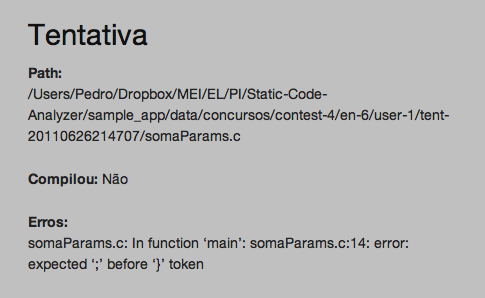
\includegraphics[width=0.8\textwidth]{imagens/erros.png}
\end{center}
\end{figure}

\end{frame}

\subsection{Adição de funcionalidades}
\begin{frame} \frametitle{Adição de funcionalidades}
Preparação do sistema para:
\begin{itemize}
\item gerar relatório dos resultados e de métricas para determinado concurso
\item permitir o download ou a visualização dentro do browser dos relatórios
\end{itemize}

\begin{figure}[h]
\begin{center}

\includegraphics[width=0.8\textwidth]{imagens/concurso.png}
\end{center}
\end{figure}

\end{frame}

\begin{frame} \frametitle{Gerar relatório de resultados}
\begin{itemize}
\item Ir à tabela de melhores resultados e ir buscar todas as entradas para o concurso em questão
\item Para cada utilizador encontrar o resultado de cada enunciado
\item Apenas contar os que estiverem 100\% correctos
\item Calcular o resultado de cada enunciado, tendo em conta o seu peso no concurso
\item Apresentar o resultado calculado e o tempo de execução
\end{itemize}
\end{frame}

\begin{frame} \frametitle{Relatório de resultados}
\begin{figure}[h]
\begin{center}
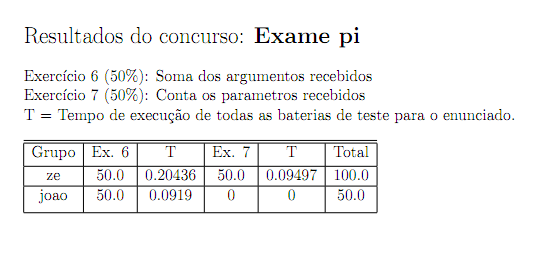
\includegraphics[scale=0.5]{imagens/relatorio.png}
\end{center}
\end{figure}
\end{frame}


\section{Metricas}
\begin{frame} \frametitle{Metricas Implementadas}
\begin{itemize}
\item Grafo de includes do sistema e de cada ficheiro
\item Nr linhas de comentários (que não são pedaços de código comentados)
\item Densidade de comentários
\item Index de Mccabe
\item NLOC (nr de linhas do pretty print)
\item Nr de linhas fisicas
\item Clones por bloco
\item Assinaturas de funções e nomes de funções
\end{itemize}
\end{frame}

\begin{frame}[fragile] \frametitle{Metrics Datatypes}
\begin{haskellcode}
type Metrics = M.Map MetricName MetricValue
type MetricName = (String, Maybe FileSrc,Maybe FunctionName)
data MetricValue =
    | Num Double
    | Clone (M.Map FileDst [(Ocurrency, LineSrc, LineDst)])
    | Includes ([SystemIncludes],[Includes])
    | FunSig [FunSignature]
    | Graphviz DotFile
    | GraphvizProject DotFile																				 
\end{haskellcode}
\end{frame}

\newcommand{\metricsins}{\mathbin{>\mkern-7mu\circ\mkern-9mu>}}
\newcommand{\metricscat}{\mathbin{>\mkern-7mu+\mkern-11mu>}}
\begin{frame}[fragile] \frametitle{Metrics API}
\begin{haskellcode}
(>.>) :: Metrics -> (MetricName,MetricValue) -> Metrics
m >.> (mn,mv) = 
    case M.lookup mn m of
        Nothing    -> m'
        (Just mv') -> if mv' == mv then m else m'
    where m' = M.insert mn mv m
\end{haskellcode}
\begin{block}{Caso de uso}
$emptyMetrics~\metricsins~(("mccbaIndex",Nothing,Nothing), Num~10)$
\end{block}
\end{frame}

\begin{frame}[fragile] \frametitle{Metrics API}
\begin{haskellcode}
(>+>) :: Metrics -> Metrics -> Metrics
m1 >+> m2 = M.union m1 m2
\end{haskellcode}
\begin{block}{Caso de uso}
\begin{haskellcode}
concatMetrics :: [Metrics] -> Metrics
concatMetrics = foldl (>+>) emptyMetrics
\end{haskellcode}
\end{block}
\end{frame}

\begin{frame}[fragile] \frametitle{Metrics API}
\begin{haskellcode}
foldrM :: (MetricName -> MetricValue -> c -> c) -> c -> Metrics -> c
foldrM f s = M.foldrWithKey f s
\end{haskellcode}
\begin{block}{Caso de uso}
\begin{haskellcode}
...
foldrM step noop m
    where step k v r =  "\\begin{dot2tex}[]"
                  >> (fromString $ fromGraphvizP v)
                  >> "\\end{dot2tex}"
                // r
          fromGraphvizP (GraphvizProject l) = l
\end{haskellcode}
\end{block}
\end{frame}

\begin{frame}[fragile] \frametitle{Metrics API}
\begin{haskellcode}
getMetricsFrom :: (a -> IO Metrics) -> [a] -> IO Metrics
getMetricsFrom f l =
    forkMapM f l >>=
        return . concatMetrics . map (either (const emptyMetrics) id)
\end{haskellcode}
\begin{block}{Caso de uso}
\begin{haskellcode}
getListOfCFiles :: FilePath -> IO [FilePath]
getTreeFromFile :: FilePath -> [FilePath] -> IO [(FilePath,CTranslUnit)]
mccabePerFun :: (FilePath,CTranslUnit) -> IO Metrics

getListOfCFiles fp >>= getTreeFromFile fp >>= getMetricsFrom mccabePerFun
\end{haskellcode}
\end{block}
\end{frame}

\begin{frame}[fragile] \frametitle{Implementação}
\begin{block}{}
\begin{haskellcode}
mccabeIndex :: Data a => a -> IO Int
mccabeIndex = applyTU (full_tdTU typesOfInstr)

typesOfInstr = constTU 0
  `adhocTU` loop
  `adhocTU` binaryOp
loop :: CStat -> IO Int
loop = return . loop_
  where loop_ (CIf _ _ _ _)    = 1
        loop_ (CSwitch _ _ _)  = 1
        loop_ (CWhile _ _ _ _) = 1
        loop_ (CFor _ _ _ _ _) = 1
        loop_ _                = 0
        binaryOp :: CBinaryOp -> IO Int
        binaryOp = return . binaryOp_
          where binaryOp_ CLndOp = 1
                binaryOp_ CLorOp  = 1
                binaryOp_ _      = 0
\end{haskellcode}
\end{block}
\end{frame}

\begin{frame}[fragile] \frametitle{Implementação}
\begin{block}{}
\begin{haskellcode}
ncloc :: (FilePath,CTranslUnit) -> IO Metrics
ncloc (file,tree) =
  let len = (length . filter (not . null) . lines . show . pretty) tree
  in return $ emptyMetrics
       >.> (("ncloc",Just file,Nothing),Num $ fromIntegral len)
\end{haskellcode}
\end{block}
\end{frame}

\section{Conclusão e trabalho futuro}
\begin{frame} \frametitle{Conclusão e trabalho futuro}
\begin{itemize}
\item Todas as metricas pretendidas foram implementadas
\item Foi desenvolvida uma api para o sistema de extracção de metricas 
\item Sistema preparado para extracção de qualidade de um programa através das metricas calculadas
\item Ambas as interfaces de comunicação com a aplicação (Web e linha de comandos) ficaram terminadas
\item São gerados relatórios sobre os resultados de cada utilizador nos concursos, e sobre as métricas
\end{itemize}
\end{frame}

\begin{frame} \frametitle{Perguntas}
\begin{center}\huge{?}\end{center}
\end{frame}

\end{document}
